%% =====================================================================
%%  Physics-Informed Inverse Calibration of the Double-Heston Model
%%  for Stable Option-Surface Parameter Recovery
%%
%%  Springer LNCS / LNNS format (llncs.cls).
%%  Self-contained: llncs.cls and all six figures ship with this project.
%%  Compile with pdfLaTeX. No .bib file and no bibtex run are required;
%%  the reference list is a plain thebibliography environment.
%% =====================================================================
\documentclass[runningheads]{llncs}

\usepackage{graphicx}
\usepackage{amsmath}
\usepackage{amssymb}
\usepackage{booktabs}
\usepackage{url}

% --- Float placement: keep figures near their first reference ---------
\IfFileExists{placeins.sty}{\usepackage{placeins}}{\providecommand{\FloatBarrier}{}}
\renewcommand{\topfraction}{0.90}
\renewcommand{\bottomfraction}{0.90}
\renewcommand{\textfraction}{0.07}
\renewcommand{\floatpagefraction}{0.75}
\setcounter{topnumber}{3}
\setcounter{bottomnumber}{3}
\setcounter{totalnumber}{5}

\begin{document}

\title{Physics-Informed Inverse Calibration of the Double-Heston Model
for Stable Option-Surface Parameter Recovery}

\titlerunning{Physics-Informed Inverse Calibration of the Double-Heston Model}

\author{%
Dhruva Ambhaikar\inst{1}\orcidID{0009-0008-1823-7221} \and
Dhurva Bamb\inst{1}\orcidID{0009-0003-5413-1890} \and
Viraj Choudhary\inst{1}\orcidID{0009-0005-9782-8246} \and
Kapil Rathor\inst{1}\orcidID{0000-0002-7630-3118} \and
Anagha Raich\inst{1}}

\authorrunning{D. Ambhaikar et al.}

\institute{Department of Artificial Intelligence,\\
Mukesh Patel School of Technology Management and Engineering,\\
SVKM's NMIMS, Mumbai, India}

\maketitle

\begin{abstract}
We report an internally specified held-out comparison of a
maturity-dependent Black benchmark, Heston and independent-factor
Double Heston on 16,186 reported option observations from Bitcoin,
Ether, Solana, XRP and Hyperliquid on Deribit. Model parameters were
fitted separately for each sampled date, and the primary evaluation
withheld entire expiries. A reported one-sided cluster-level Wilcoxon
test and a cluster-bootstrap lower bound both had to support a
directional improvement. For Bitcoin shock dates, median held-out
implied-volatility RMSE was 8.13, 2.50 and 1.86 volatility points for
the three models, respectively. Relative to Single Heston, the declared
criterion is met for Bitcoin and Ether but not for Solana, XRP or
Hyperliquid. Across these five markets, this pattern coincides with
greater median maturity coverage for Bitcoin and Ether; it is not a
causal estimate or proof of parameter identifiability. This manuscript
documents direct numerical model calibration and a comparative
empirical benchmark. It does not report training or evaluation of a
physics-informed neural inverse map or demonstrate stable recovery of a
unique Double-Heston parameter vector.

\keywords{Stochastic volatility \and Double Heston \and Cryptocurrency
options \and Held-out maturity evaluation \and Calibration}
\end{abstract}

% =====================================================================
\section{Introduction}
\label{sec:intro}

Anyone pricing options must decide how much structure to buy. The
Black--Scholes formula assumes a single constant volatility and is wrong
in a way every practitioner can see: implied volatility varies with both
strike and maturity. The Heston model replaces that constant with one
mean-reverting variance process and captures much of the variation. A
natural next step is to add a second variance process on a different
time scale, which is what the Double-Heston model does. The motivation
is intuitive. Short-dated options respond to volatility that
mean-reverts quickly, long-dated options to a slower component, and one
process cannot be fast and slow at once.

The argument is appealing, but the extra factor is not free. It doubles
the variance parameters from five to ten, and those parameters must be
recovered from a finite set of quoted prices. If the quoted surface does
not contain enough distinct maturities, two mean-reversion speeds cannot
be told apart, and the additional flexibility buys nothing while making
calibration harder. Whether the trade is worthwhile is therefore an
empirical question, and it is a question about the data as much as about
the model.

A comparison restricted to one relatively liquid market may not reveal
when additional model complexity ceases to help. We report a three-model
comparison on five cryptocurrency markets with differing maturity
coverage. The manuscript describes date-selection rules and an
internally frozen evaluation protocol; the associated timestamped
manifest and prediction-level artifacts are needed for independent
verification.

Our contributions are:

\begin{enumerate}
\item A reported five-market comparison of a term-structure Black
benchmark, Heston and Double Heston, including withheld-expiry
evaluation and a stated directional success rule.
\item Evidence that the Double-Heston advantage over Black--Scholes is
large across the five sampled markets, while its advantage over
one-factor Heston is conditional in the observed data and occurs in the
two markets with the greatest quoted maturity coverage.
\item An assessment of maturity coverage as one possible explanation for
that pattern, while retaining the negative and inconclusive comparisons.
\item Disclosure of a defect in the Black baseline implementation and
the reported effect of its correction on the Bitcoin shock-date summary.
\end{enumerate}

We do not claim that Double Heston is the best available model, that
these results transfer to equity or foreign-exchange markets, or that
they imply a trading strategy. Our more limited finding is an
association, in these five markets, between maturity coverage and the
held-out benefit of a second variance factor. The present experiments
involve direct numerical calibration; a physics-informed neural
inverse-calibration model is not evaluated here.

% =====================================================================
\section{Related Work}
\label{sec:related}

The Black--Scholes framework \cite{ref:bs} and Merton's analysis of
rational option pricing \cite{ref:merton} establish classical
option-valuation foundations. Black's forward/futures option formulation
\cite{ref:black76} is relevant to the contract conventions considered
here. Observed variation in implied volatility across strikes and
maturities motivates models beyond constant volatility, as discussed by
Gatheral \cite{ref:gatheral}.

Heston \cite{ref:heston} introduced a tractable stochastic-volatility
model in which variance follows a correlated square-root process.
Bakshi, Cao and Chen \cite{ref:bakshi} evaluated extensions
incorporating stochastic volatility, stochastic interest rates and jumps
on S\&P 500 options, finding that their implications differ across
pricing and hedging performance. Bates \cite{ref:bates} investigated
post-crash concerns in the S\&P 500 futures-option market, while Duffie,
Pan and Singleton \cite{ref:duffie} developed transform methods for
affine jump-diffusion models. Particularly relevant to the present
comparison, Christoffersen, Heston and Jacobs \cite{ref:chj} showed how
multiple stochastic-volatility factors can better capture both the shape
and term structure of equity-index option smiles. Their work motivates
testing whether a second variance factor provides a measurable benefit
beyond a one-factor model; it does not, by itself, establish that such a
benefit holds across cryptocurrency markets.

Efficient evaluation and stable calibration are essential for making
this comparison meaningful. Carr and Madan \cite{ref:carrmadan}
introduced FFT valuation of options, and Fang and Oosterlee
\cite{ref:fangoost} introduced Fourier-cosine expansions. Lord and Kahl
\cite{ref:lordkahl} investigated the treatment of complex logarithms in
Heston-like characteristic functions, while Cui, del Ba\~{n}o Rollin and
Germano \cite{ref:cui} studied efficient Heston calibration. Feller's
work on singular diffusion boundaries \cite{ref:feller} provides
background for the treatment of the square-root variance boundary;
whether a Feller constraint is imposed is a separate modelling and
calibration choice.

Cryptocurrency options present an important empirical setting for this
question. Madan, Reyners and Schoutens \cite{ref:madan} compared several
calibrated models, including Black--Scholes, variance-gamma-related
models and Heston, using Bitcoin option data. Lian and Chen
\cite{ref:lian} examined cryptocurrency derivatives under a distinct
two-factor, state-dependent stochastic-volatility framework with jumps.
Hou and coauthors \cite{ref:hou} investigated cryptocurrency-option
pricing with stochastic volatility and correlated jumps, highlighting
the role of jumps and co-jumps. Alexander and Imeraj \cite{ref:ai2021}
constructed Bitcoin implied-volatility indices from Deribit option
observations and examined the associated variance risk premia; their
subsequent study \cite{ref:ai2023} evaluated dynamic delta hedging with
smile-adjusted measures. These studies establish relevant cryptocurrency
option-pricing and volatility dynamics, but they do not directly answer
the specific question considered here: how the held-out benefit of a
second Heston variance factor changes across several cryptocurrency
markets with different maturity coverage.

Physics-informed neural networks combine governing-equation information
with supervised observations \cite{ref:raissi}. Hainaut and Casas
\cite{ref:hainaut} investigated physics-inspired neural pricing under
single-factor Heston, while Zhang and coauthors \cite{ref:zhang} studied
differential-network-assisted Heston calibration. These are related
motivations, not methods implemented in the present numerical
three-model benchmark; evidence for a learned inverse map would require
additional methods and recovery experiments.

Our evaluation therefore compares a term-structure Black baseline,
single-factor Heston and two-factor Heston using predefined calibration
and held-out partitions, including withholding entire expiries. Because
multiple dates may belong to the same market episode, paired comparisons
are evaluated at the cluster level. Wilcoxon's signed-rank procedure
\cite{ref:wilcoxon}, bootstrap inference \cite{ref:efron} and
clustered-resampling methodology \cite{ref:cameron} motivate the stated
statistical checks. The stated protocol follows the motivation for
advance specification \cite{ref:nosek}; Section~\ref{sec:data} describes
the reported internal freeze. The published manuscript does not provide
an independently timestamped registry record, so we do not call it
externally preregistered.

% =====================================================================
\section{Models and Numerical Method}
\label{sec:models}

All models are evaluated on a common undiscounted, forward-normalised
basis. Let $F$ be the expiry forward, $K$ the strike, $x = \log(F/K)$
the log-forward moneyness and $\tau$ the time to maturity in years. If
$C_{\mathrm{undisc}}$ is a call value in the common quote currency after
contract-multiplier and settlement-currency conversion, we use
$c = C_{\mathrm{undisc}}/F$. For a conventionally discounted currency
price $C_{\mathrm{disc}}$ and discount factor $D$, the equivalent
normalisation is $C_{\mathrm{disc}}/(DF)$. Plotting $C/K$ versus $F/K$
is a separate strike-normalised display; it must not be mistaken for the
calibrated $C/F$ scale. The manuscript's available data do not specify
the precise exchange-rate snapshot and contract-multiplier conversions
used; these must be verified from the source implementation.

\subsection{Black--Scholes with a Term Structure}
\label{sec:bs}

The constant-volatility model is given one volatility per expiry rather
than one for the whole surface. This is a deliberately generous
baseline: it absorbs the entire maturity dimension of the smile and
leaves only the strike dimension unexplained. A quote in a calibrated
expiry is priced with that expiry's volatility; a quote in a withheld
expiry is priced by interpolating total variance linearly between
neighbouring calibrated expiries, with a flat extension beyond them.

\subsection{Heston and Double Heston}
\label{sec:heston}

The one-factor model is
\begin{align}
\frac{dF}{F} &= \sqrt{v}\, dW_1, \\
dv &= \kappa(\theta - v)\, dt + \sigma \sqrt{v}\, dW_2,
\qquad \mathrm{corr}(dW_1, dW_2) = \rho,
\end{align}
with five parameters $(\kappa, \theta, \sigma, \rho, v_0)$. Here
$\kappa$ is the speed at which variance returns to its long-run level
$\theta$, $\sigma$ is the volatility of variance, $\rho$ couples spot
and variance shocks and produces the skew, and $v_0$ is the variance
today.

The Double-Heston model drives the same underlying with two independent
square-root processes,
\begin{align}
\frac{dF}{F} &= \sqrt{v_1}\, dW_1 + \sqrt{v_2}\, dW_3, \\
dv_i &= \kappa_i(\theta_i - v_i)\, dt + \sigma_i \sqrt{v_i}\, dW_{2i},
\qquad i = 1, 2,
\end{align}
with $\mathrm{corr}(dW_1, dW_2) = \rho_1$ and
$\mathrm{corr}(dW_3, dW_4) = \rho_2$, and zero cross-pair Brownian
correlations, so the two factor pairs are independent. This gives ten
parameters, $(\kappa_i, \theta_i, \sigma_i, \rho_i, v_{i,0})$ for
$i = 1, 2$. The intended division of labour is that one factor reverts
quickly and governs short-dated options while the other reverts slowly
and governs long-dated ones. Because the factors are independent, the
characteristic function of the log-forward is the product of the two
single-factor characteristic functions, although actual runtime depends
on the implementation and numerical solver.

\subsection{Numerical Reference}
\label{sec:numerical}

Prices are obtained by Gauss--Laguerre inversion of the characteristic
function using a parameterisation that avoids branch-cut discontinuities
\cite{ref:lordkahl}. A 128-node result is checked against a 96-node
result; if the two disagree by more than $10^{-7}$, or a no-arbitrage
price bound is violated, the code falls back to independent adaptive
quadrature rather than clipping the value. The implementation is
described as counting fallbacks; this manuscript does not include the
resulting count, which must be obtained from its logs.

% =====================================================================
\section{Data and Pre-Specified Design}
\label{sec:data}

\subsection{Markets}
\label{sec:markets}

We use observations attributed to Deribit. Bitcoin and Ether options use
inverse, coin-denominated premium conventions; Solana, XRP and
Hyperliquid are reported as USDC-linear contracts. The premium must
first be converted to a common currency and per-unit contract basis
before price-error or normalised price comparisons. The original
quote/forward reconstruction and conversion scripts are needed to audit
those steps. Table~\ref{tab:markets} summarises the reported data. The
HYPE dates must also be checked against its actual option listing
window.

\begin{table}[htbp]
\caption{Markets, data volume and surface richness. Option observations is
the total number of quotes on the evaluated surfaces; the primary Design~B
held-out subset is smaller, 5,214 quotes in total (BTC 2,223, ETH 1,509,
SOL 658, XRP 269, HYPE 555). Expiries per day is the median number of distinct
expiries quoted on an evaluation date. A date enters the sample only if it
quotes at least five distinct expiries for Bitcoin and Ether and at least four
for the other three markets; this threshold is itself market-dependent and is
discussed in Section~\ref{sec:limitations}.}
\label{tab:markets}
\centering
\begin{tabular}{llrrr}
\toprule
Asset & Contract & Dates & Option observations & Expiries/day \\
\midrule
Bitcoin (BTC)      & Inverse, coin-settled &  66 &  6,171 & 7 \\
Ether (ETH)        & Inverse, coin-settled &  53 &  3,619 & 6 \\
Solana (SOL)       & Linear, USDC          &  32 &  2,687 & 4 \\
XRP                & Linear, USDC          &  26 &  1,249 & 4 \\
Hyperliquid (HYPE) & Linear, USDC          &  55 &  2,460 & 4 \\
\midrule
Total              &                       & 232 & 16,186 &   \\
\bottomrule
\end{tabular}
\end{table}

\subsection{Reported Date Selection and Internal Protocol Freeze}
\label{sec:selection}

The supplied draft describes the following selection protocol. For
Bitcoin and Ether we used the venue's DVOL volatility index. A shock
onset is a day on which DVOL exceeds 1.2 times its median over the
previous 60 days, de-duplicated so that onsets cannot fall within 20
days of each other; we then evaluate the surfaces 1, 4 and 8 days after
each onset. Calm dates are days on which the index sits within 5\% of
its 60-day median, at least 20 days from any onset, sampled with a fixed
random seed.

No volatility index is published for Solana, XRP or Hyperliquid. For
those we used the annualised standard deviation of the last ten daily
log returns of the perpetual contract, with a shock threshold of 1.5.
Hyperliquid options have too short a history for an episode design, so
every calendar day in the listing window is an evaluation date.

The authors report that the rules, random seeds and selection windows
were recorded and hashed before options were fetched; the internal
manifest contains
\texttt{option\_data\_fetched\_before\_freeze:\ false}. A timestamped
freeze record, its hash, the first options-fetch time and the full
excluded-date manifest are required for independent verification. This
should not be confused with independent registry-based preregistration.

\subsection{Calibration and Held-Out Evaluation}
\label{sec:calibration}

Each model is calibrated independently on each date, minimising a
vega-weighted squared pricing error, with twelve restarts for the Heston
models to reduce the risk of a local optimum. Two held-out designs were
fixed in advance. Design~A withholds a random subset of quotes from
every expiry. Design~B withholds entire expiries, so a model must price
a maturity it has never seen. Design~B is the primary endpoint, because
it tests the maturity structure directly, which is exactly where a
second variance factor should help. Table~\ref{tab:results} reports
Design~B; Design~A is not tabulated here and no claim about its
cell-level agreement is made. Accuracy is reported as the
root-mean-square error in implied-volatility points on held-out quotes,
which is comparable across strikes and maturities.

\subsection{Reported Directional Success Criterion}
\label{sec:criterion}

Dates are not independent: several can belong to one volatility episode.
We therefore cluster by episode (by ISO week for Hyperliquid) and
require both of the following before declaring that one model beats
another: a one-sided Wilcoxon signed-rank test over clusters with
$p < 0.05$, and a cluster-bootstrap 95\% lower bound on the mean paired
difference strictly above zero, using 5,000 replicates and a fixed seed.
The two procedures are complementary checks on the same cluster data,
not independent tests. The nine rows in Table~\ref{tab:results} were not accompanied by a
familywise multiplicity adjustment fixed in advance, so we report the effect
of applying one after the fact. Under Holm--Bonferroni at $\alpha=0.05$ the
four cells declared as wins (both Bitcoin rows and both Ether rows) remain
significant and the five undeclared cells remain non-significant;
Benjamini--Hochberg control of the false discovery rate at $q=0.05$ yields the
same four discoveries. The classification is therefore unchanged by
multiplicity adjustment. Note also that with ten episode clusters the smallest
attainable one-sided Wilcoxon $p$-value is $2^{-10}=0.00098$, so the Bitcoin
and Ether shock rows sit at the floor of what the test can report rather than
at an unusually extreme value. Two rows pass only the reported Wilcoxon
check.

\subsection{Disclosure of a Defect in Our Own Baseline}
\label{sec:defect}

After the Bitcoin results were produced we found a defect in our
Black--Scholes implementation. Because each quote's maturity was
computed from its own trade timestamp, quotes in one expiry had
marginally different maturities, and the routine intended to place one
volatility per expiry in fact placed one volatility per quote. The
baseline therefore reproduced its own calibration quotes exactly and
interpolated between individual quotes rather than between expiries.

The authors report recording the correction before applying it and
retaining the original outputs. The reported corrected Black median
held-out error on Bitcoin shock dates changes from 9.63 to 8.13
volatility points. All Black entries in Table~\ref{tab:results} are
labelled as the corrected implementation. The full before/after artifact
is not supplied in this manuscript, so we do not claim to reproduce it
here. The Heston implementations do not use the affected expiry knots.

% =====================================================================
\section{Results}
\label{sec:results}

\subsection{Double Heston Against Black--Scholes}
\label{sec:vsbs}

The displayed medians favour Double Heston over the maturity-dependent
Black baseline in every reported asset/regime row;
Table~\ref{tab:results} does not report the corresponding
Black-versus-Double cluster-level tests. On Bitcoin shock dates the
median held-out error falls from 8.13 to 1.86 volatility points, a
reduction of about 77\%. The paired difference is positive on 29 of 29
dates and in 10 of 10 episodes, with a cluster-bootstrap interval of
[5.22, 8.31] volatility points. This comparison is descriptive unless
the full paired Black-versus-Double testing outputs are supplied.

\subsection{Double Heston Against One-Factor Heston}
\label{sec:vssh}

Here the five markets divide cleanly into two groups
(Table~\ref{tab:results}).

On Bitcoin the two-factor model wins in both regimes. On shock dates the
mean advantage is 0.57 volatility points, positive on 23 of 29 dates and
in all 10 episodes, with $p = 0.001$ and an interval of [0.39, 0.71]. On
calm dates the advantage is larger at 1.11 points, with an interval of
[0.64, 1.65].

On Ether it also wins in both regimes. The advantage is 0.96 points on
shock dates ([0.61, 1.46]), and 0.53 on calm dates ([0.22, 0.86]).

On Solana, XRP and Hyperliquid it does not meet the declared criterion
in any cell. On Solana calm dates the mean paired difference favours
Single Heston ($-0.48$ points; bootstrap interval $[-0.98, -0.02]$).
However, the reported one-sided Wilcoxon $p = 0.839$ tests the
Double-Heston direction; a separate, appropriately specified
reverse-direction confirmation is not reported, so this row is not
labelled a confirmed Single-Heston win. On XRP shock dates the Wilcoxon
test passes ($p = 0.037$) but the bootstrap interval $[-0.08, 1.82]$
contains zero, so the stated dual criterion is not met. Hyperliquid
shows the same pattern, $p = 0.029$ with an interval of
$[-0.06, 0.74]$. The latter two rows illustrate why the reported
two-part criterion matters: the one-sided Wilcoxon check alone would
give a different classification.

\begin{table}[htbp]
\caption{Reported held-out accuracy and directional tests, Design~B.
BS = term-structure Black--Scholes, SH = one-factor Heston,
DH = Double Heston. The BS, SH and DH columns are medians of the
per-date held-out implied-volatility RMSE, in volatility points, and
bold marks the lower of the SH/DH pair. The SH$-$DH column is the mean
paired difference across clusters, while Wilcoxon tests paired cluster
differences; a median and a mean paired difference need not agree in
sign, as on Solana and XRP. ``Beats SH'' requires Wilcoxon $p < 0.05$
and a cluster-bootstrap 95\% lower bound above zero. The reported $p$
values are one-sided in the DH improvement direction; multiplicity
adjustment is not documented.}
\label{tab:results}
\centering
\setlength{\tabcolsep}{4pt}
\small
\begin{tabular}{llrrrrrcc}
\toprule
Asset & Regime & BS & SH & DH & SH$-$DH & $p$ & 95\% CI & Beats SH \\
\midrule
BTC  & shock &  8.13 & 2.50 & \textbf{1.86} & $+0.57$ & 0.001  & $[0.39, 0.71]$   & yes \\
BTC  & calm  &  6.40 & 2.53 & \textbf{1.37} & $+1.11$ & 0.0001 & $[0.64, 1.65]$   & yes \\
ETH  & shock &  8.76 & 3.23 & \textbf{2.32} & $+0.96$ & 0.001  & $[0.61, 1.46]$   & yes \\
ETH  & calm  &  8.77 & 2.68 & \textbf{2.34} & $+0.53$ & 0.0026 & $[0.22, 0.86]$   & yes \\
SOL  & shock & 10.15 & 3.82 & \textbf{3.67} & $+0.27$ & 0.234  & $[-0.10, 1.14]$  & no  \\
SOL  & calm  &  6.98 & 2.42 & \textbf{2.36} & $-0.48$ & 0.839  & $[-0.98, -0.02]$ & no  \\
XRP  & shock & 13.09 & \textbf{5.24} & 5.72 & $+0.59$ & 0.037  & $[-0.08, 1.82]$  & no  \\
XRP  & calm  &  7.00 & \textbf{3.28} & 3.52 & $-0.19$ & 0.727  & $[-0.71, 0.30]$  & no  \\
HYPE & all   &  4.68 & 3.61 & \textbf{3.26} & $+0.27$ & 0.029  & $[-0.06, 0.74]$  & no  \\
\bottomrule
\end{tabular}
\end{table}

\subsection{Descriptive Bitcoin Error Distributions}
\label{sec:ecdf}

Table~\ref{tab:results} reports the stated primary Design~B endpoint.
Figure~\ref{fig:errpanels} displays additional descriptive plots from a
subset labelled as 50 Bitcoin dates and 2,223 quotes;
Table~\ref{tab:markets}, by contrast, reports 66 Bitcoin evaluation
dates and 6,171 option observations. The criteria producing this smaller
plotted subset are not supplied with the manuscript. It must therefore
not be treated as a randomly representative subset of the full
benchmark. Panel (a) displays quote-level absolute IV errors, with
displayed medians of 2.95, 1.39 and 0.93 volatility points for Black,
Single Heston and Double Heston respectively. Panel (b) displays
date-level mean absolute-error advantages and uncertainty bars. These
summaries differ from the cluster-level, per-date IV-RMSE endpoint in
Table~\ref{tab:results}; neither panel constitutes an additional
confirmatory test.

\begin{figure}[htbp]
\centering
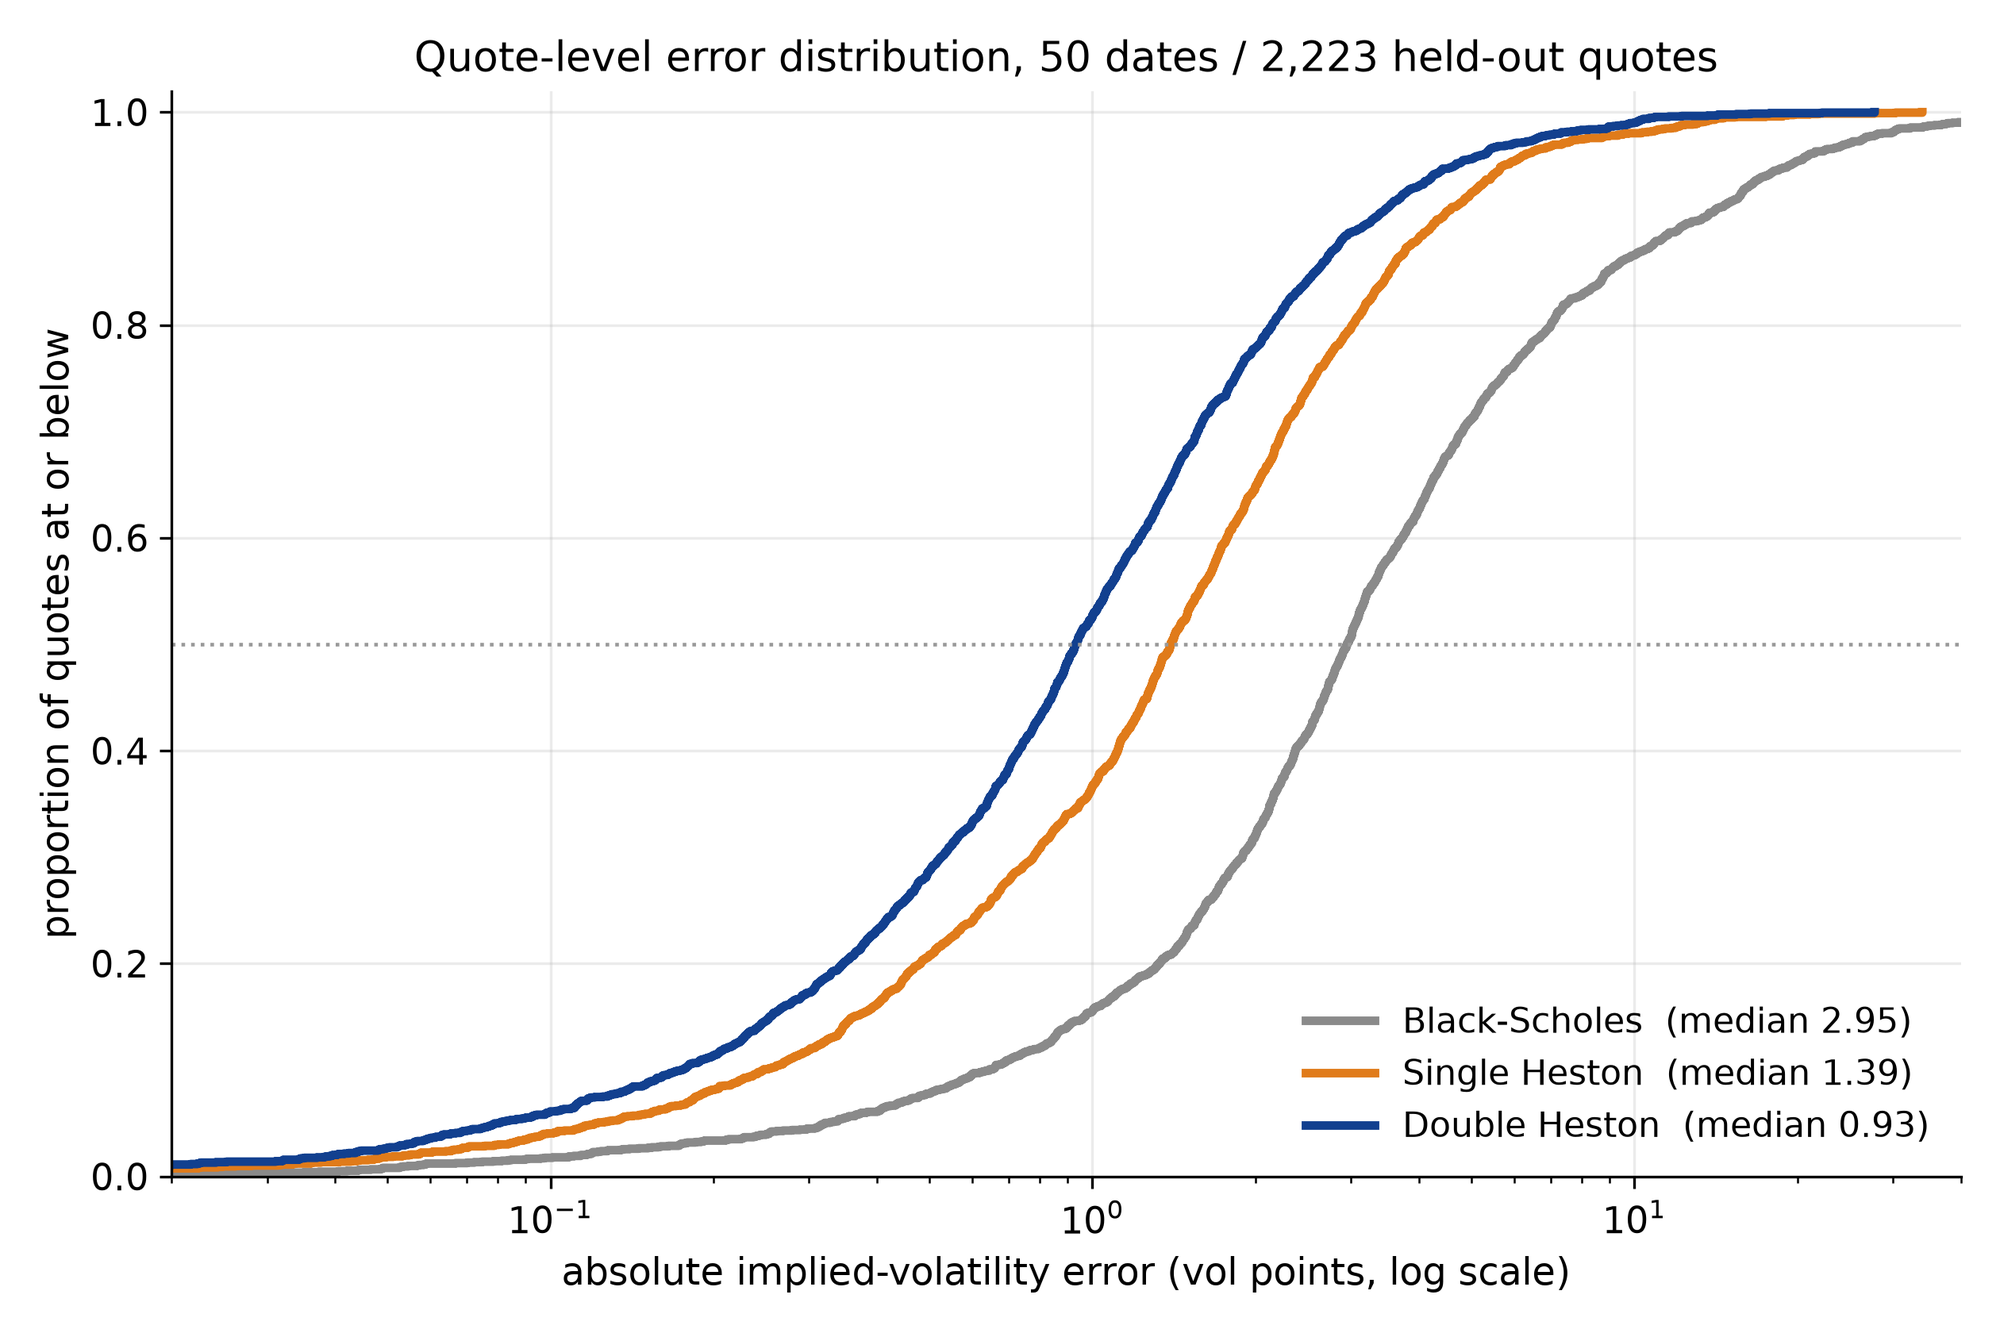
\includegraphics[width=0.88\linewidth]{fig_error_ecdf_panel.png}\\[2ex]
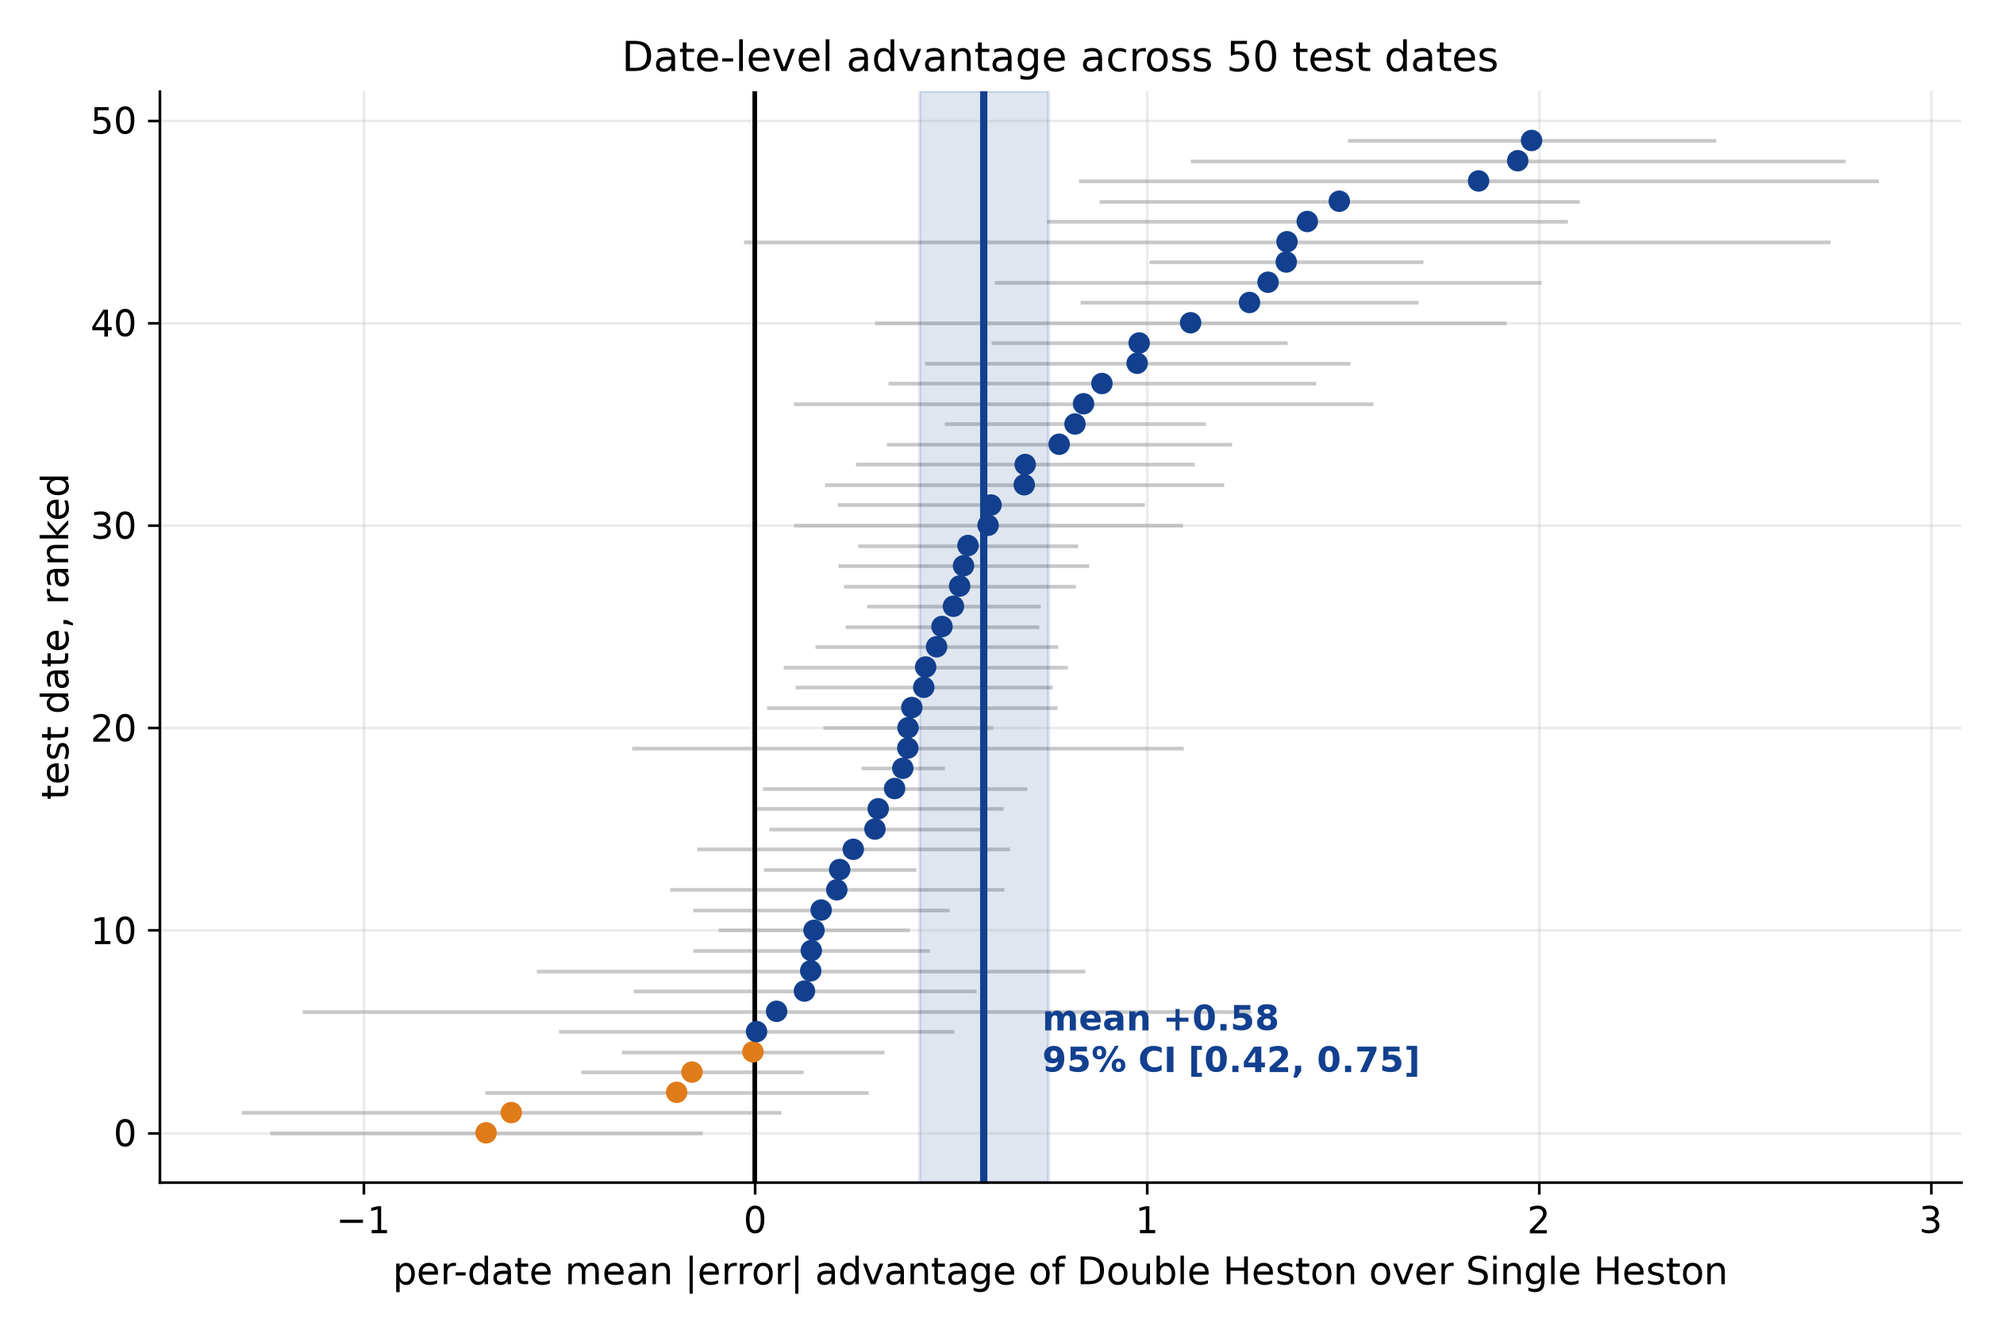
\includegraphics[width=0.88\linewidth]{fig_error_date_panel.png}
\caption{Descriptive Bitcoin plots reproduced as larger panels from the
supplied composite source: (a) empirical cumulative distribution of
quote-level absolute implied-volatility error; (b) ranked date-level
mean absolute-error advantage with displayed uncertainty bars. The
plotted subset contains 50 dates and 2,223 quotes, and its filtering
rule remains to be documented.}
\label{fig:errpanels}
\end{figure}

\FloatBarrier

\subsection{The Pattern Behind the Split}
\label{sec:pattern}

The division is not random with respect to market structure.
Table~\ref{tab:markets} reports the median number of distinct expiries
quoted per evaluation date: Bitcoin quotes seven and Ether six, while
Solana, XRP and Hyperliquid quote about four. The two markets in which
the second variance factor pays are exactly the two that quote the most
maturities.

One possible explanation is that maturity coverage helps distinguish two
mean-reversion speeds. Four expiries, particularly when clustered at
short maturities, may offer less information about slow and fast
variance dynamics than six or seven expiries spanning a wider range. The
observed grouping is consistent with this explanation, but expiry count
is confounded with asset liquidity and market history, and direct
parameter-identifiability diagnostics were not performed.

\subsection{Illustrative Bitcoin Surfaces}
\label{sec:surfaces}

Figure~\ref{fig:surface} shows a supplied single-date Bitcoin
comparison. The plot is in strike-normalised $F/K$--$C/K$ coordinates,
not the $C/F$ training or valuation convention. It labels the plotted
RMSE values (in units of $10^{-3}$ of $C/K$) as 1.33, 1.54 and 0.28 for
Black, Single Heston and Double Heston. The annotation of a 4.7-fold
improvement follows from these rounded values. The far-right market
marker is clipped in the source image; the underlying plotting data are
needed to regenerate it with additional axis padding. The earlier draft
also contained a maturity curve with a discontinuous Black baseline near
an expiry knot, which is not explained by the continuous total-variance
interpolation described in Section~\ref{sec:bs}. That unverified plot
has been excluded from the evidentiary figure set, but its original
source image is retained in the editable project for investigation.

\begin{figure}[htbp]
\centering
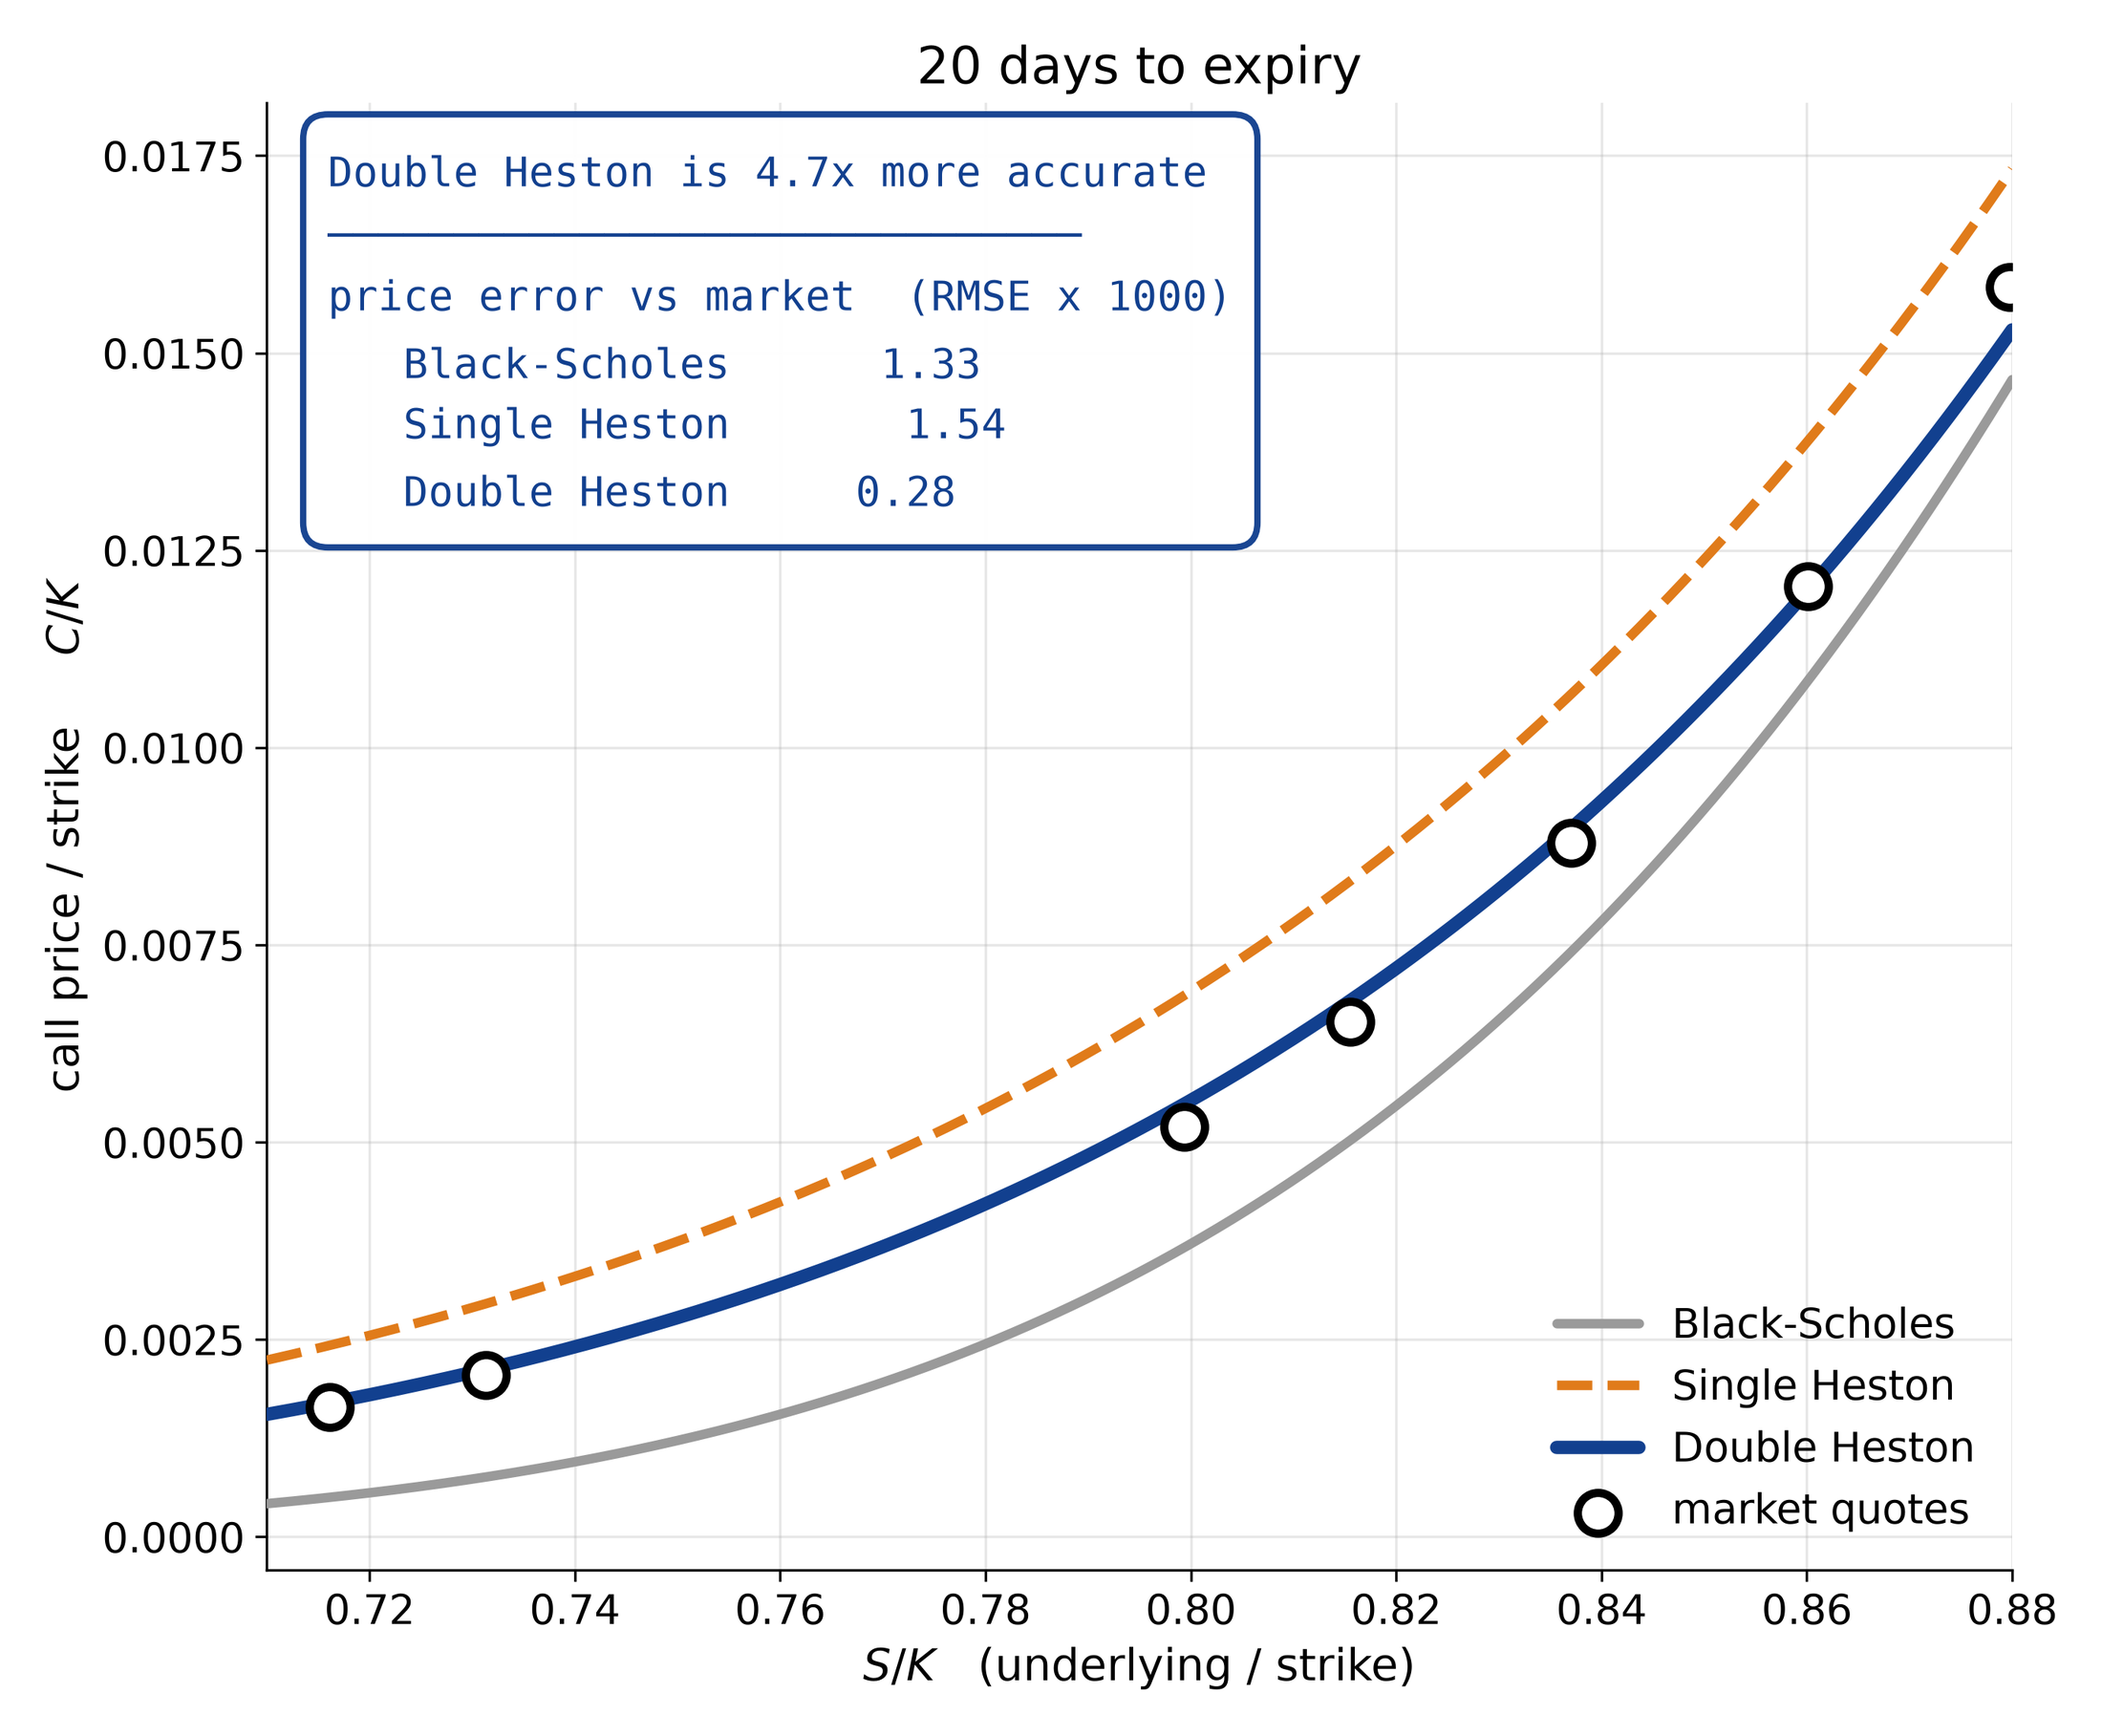
\includegraphics[width=0.82\linewidth]{fig1_C_vs_S.png}
\caption{Illustrative Bitcoin surface at one expiry (27~July 2024, the
20-day expiry), displayed in $F/K$ (horizontal) and $C/K$ (vertical)
coordinates. This expiry is ranked second of the eight quoted that day and so
belongs to the Design~B \emph{calibration} set, not the held-out set: all
three models are in-sample on the quotes shown. The error figures printed in
the panel are computed over the seven quotes inside the plotted moneyness
window rather than over all twenty in the expiry, and source-image markers
near the right plotting boundary are clipped. The figure is descriptive; the
cross-date evidence is Table~\ref{tab:results}.}
\label{fig:surface}
\end{figure}

\FloatBarrier

To show variation rather than only a favourable single-date result, the
supplied three-panel composite is reproduced as larger individual panels
in Figs.~\ref{fig:range} and~\ref{fig:worst}. The first is the supplied
date with largest DH advantage, the second a median-advantage example,
and the third the largest SH advantage. The source composite's headline
of 42/50 DH-positive dates uses a per-date RMSE comparison, whereas the
other Bitcoin diagnostic uses mean absolute errors. These are not
interchangeable, and the exact counts must be reconciled from the
date-level outputs. The cropped panels preserve all source data markers
and their original legends; the contested composite headline is not
repeated as a verified manuscript claim.

\begin{figure}[htbp]
\centering
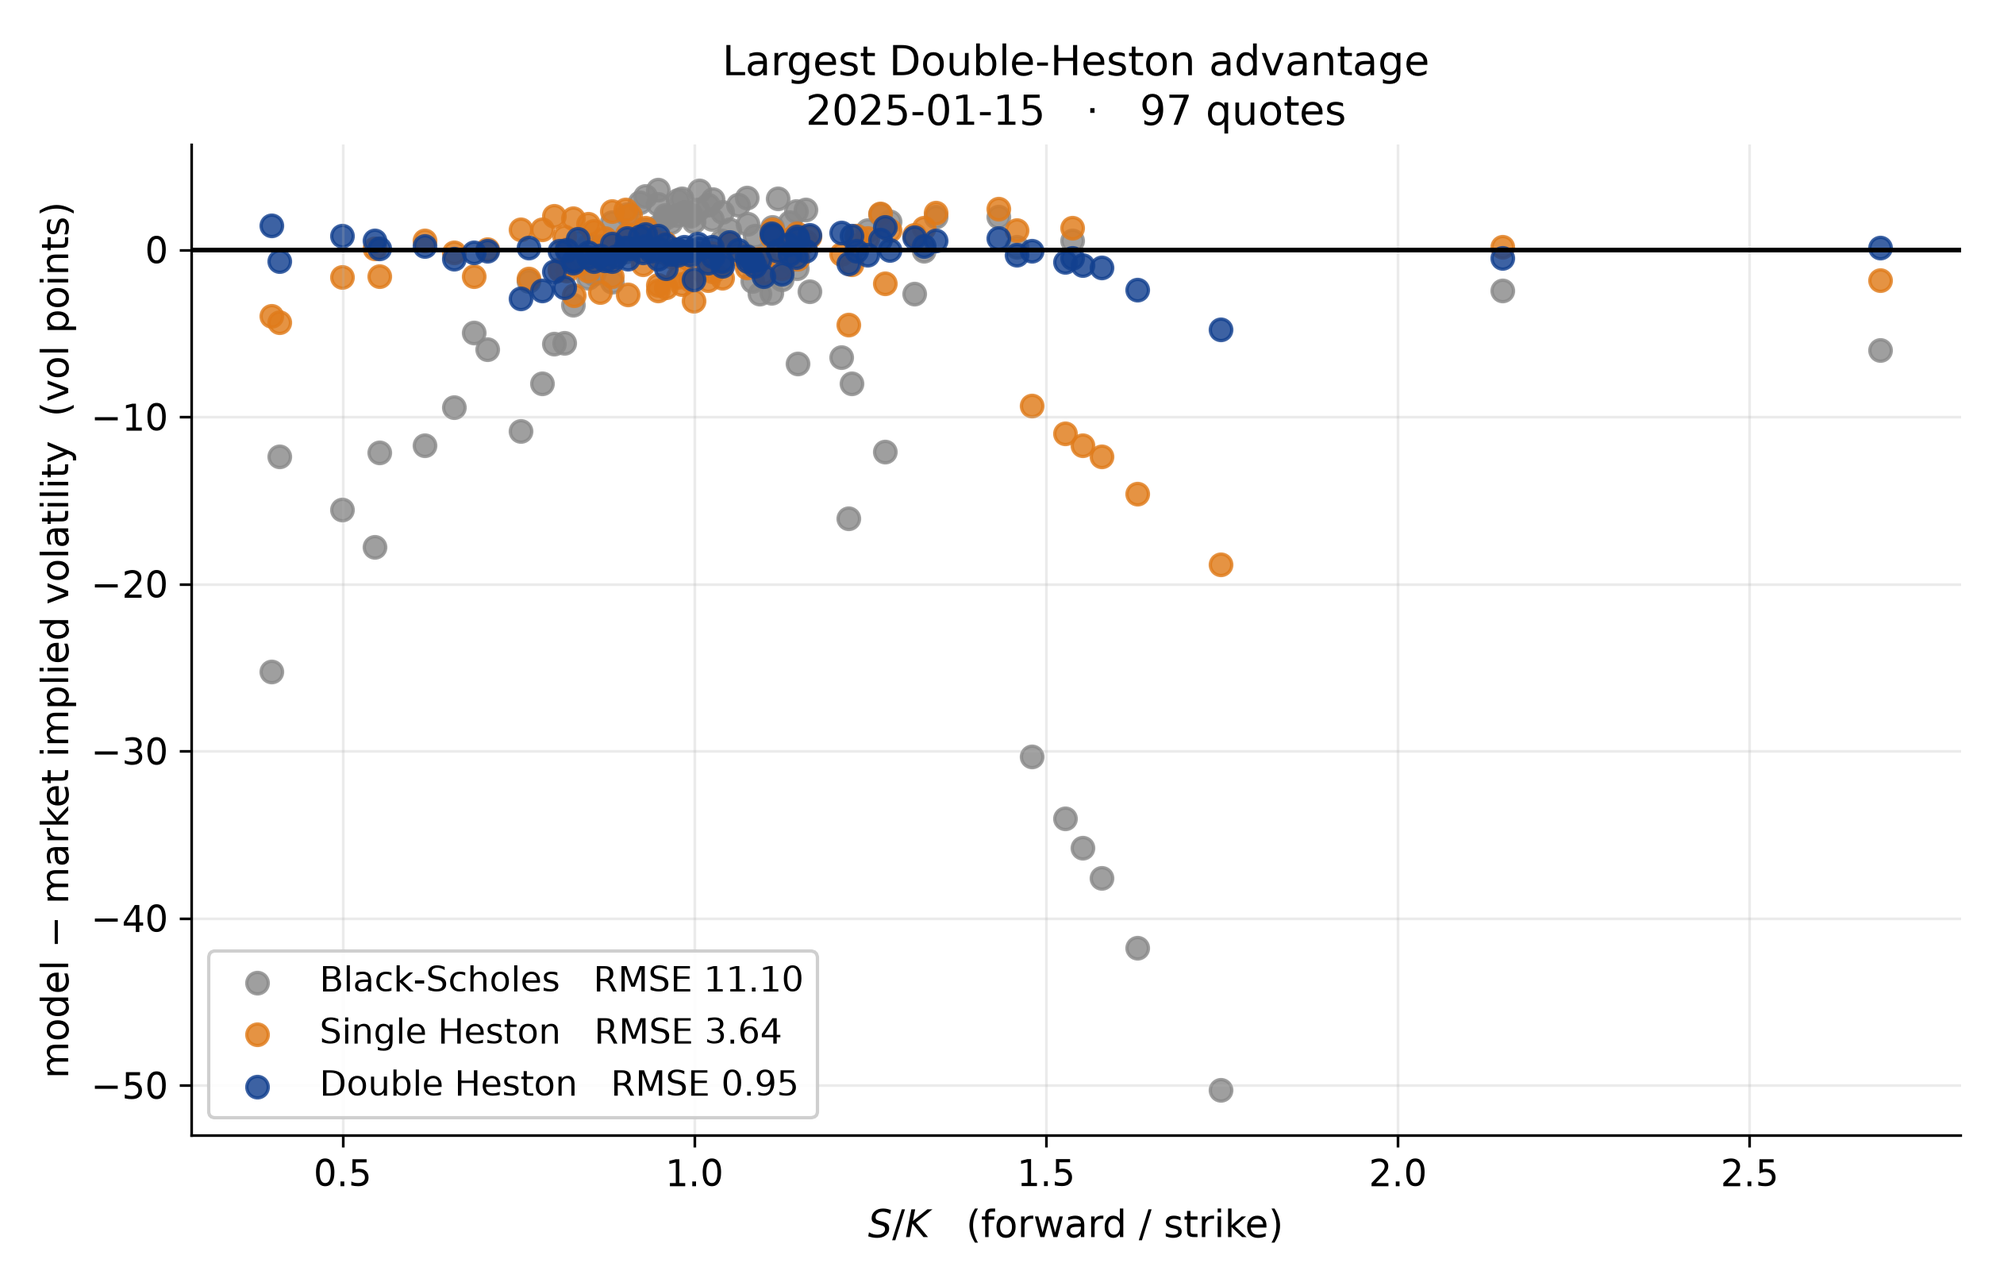
\includegraphics[width=0.88\linewidth]{fig_range_best.png}\\[2ex]
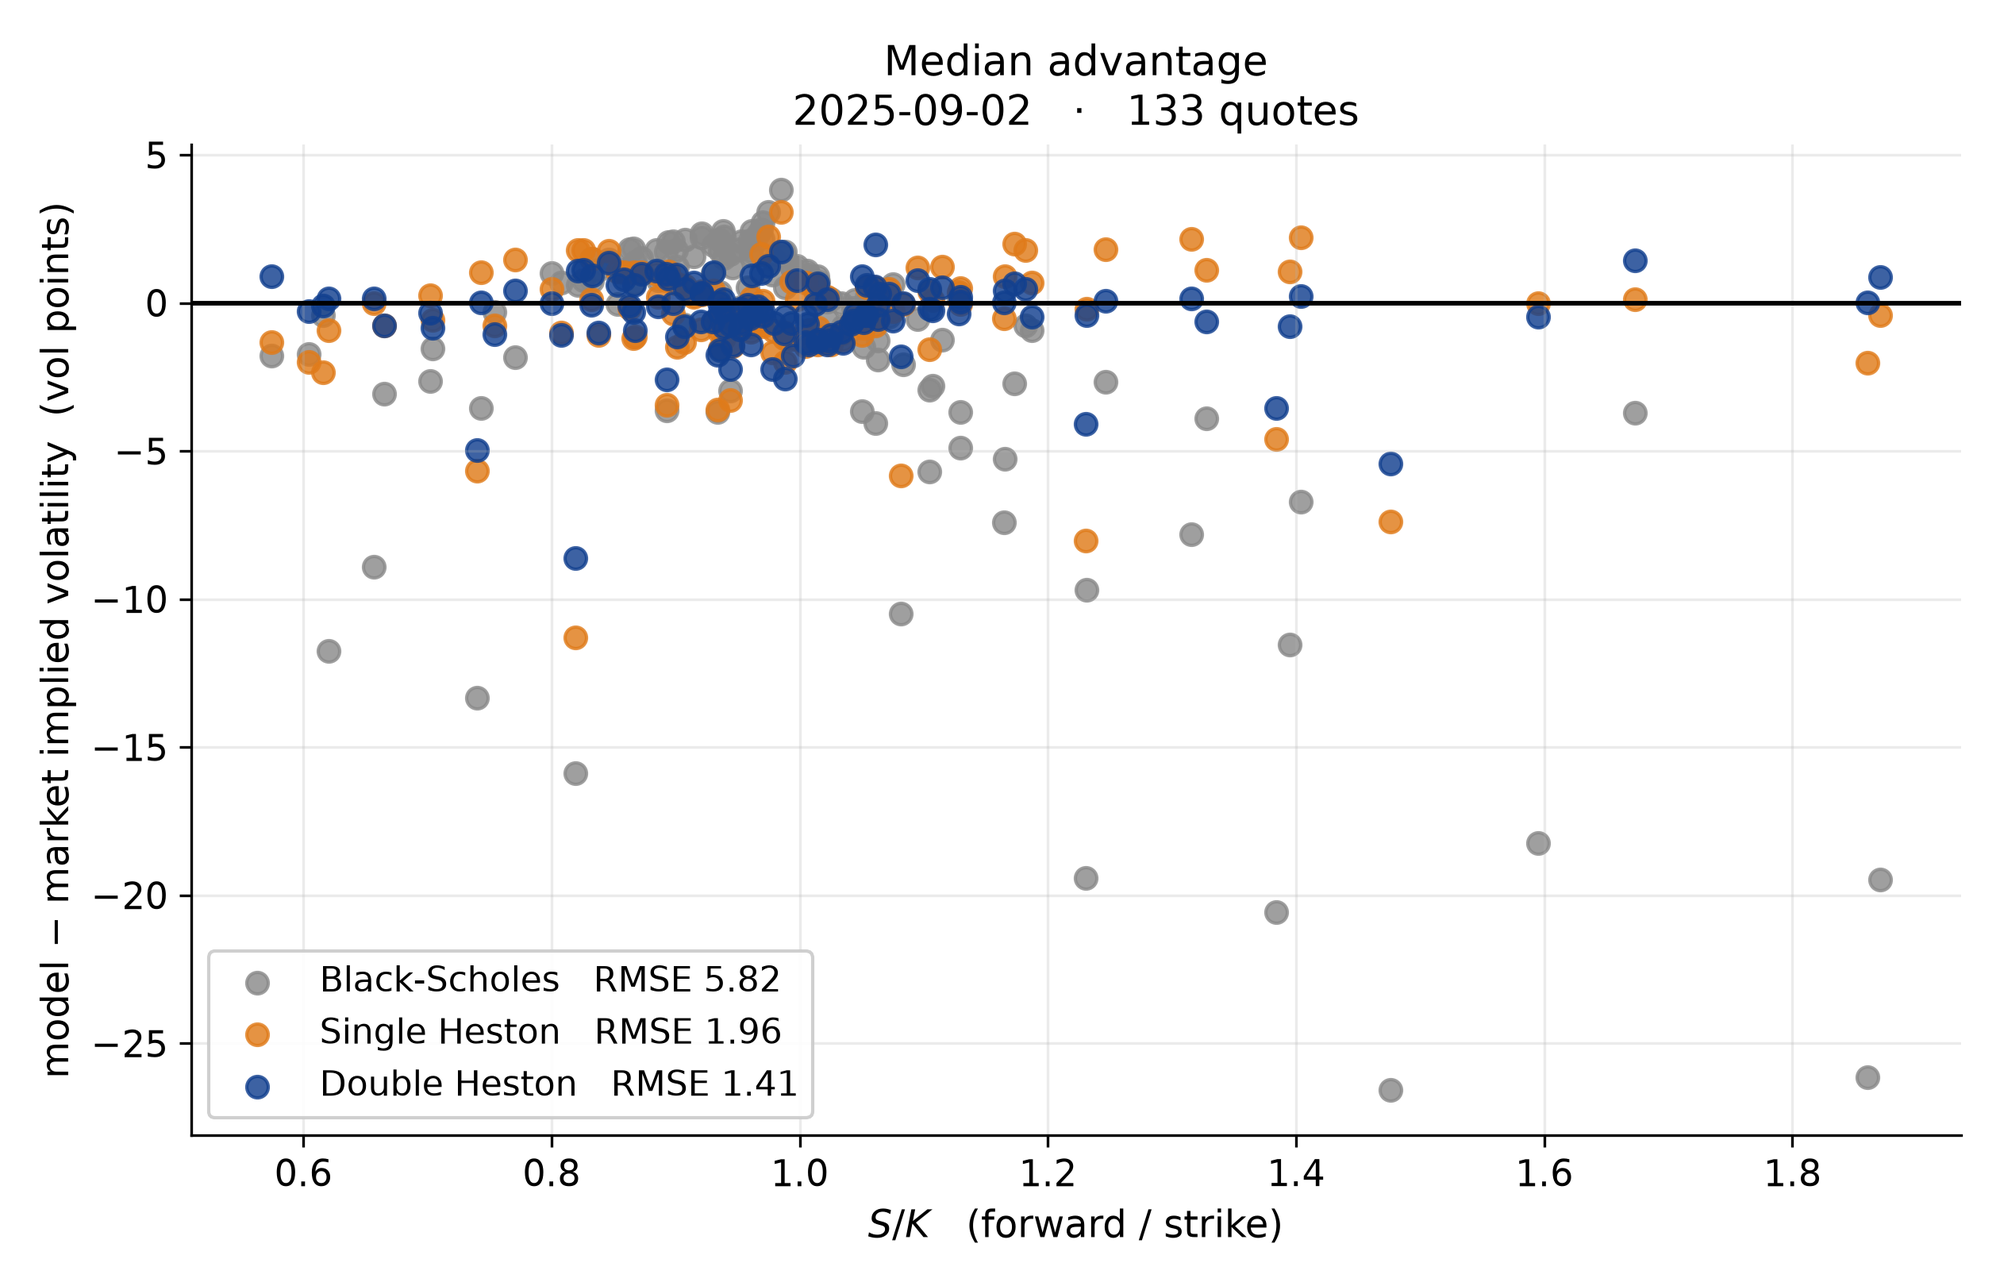
\includegraphics[width=0.88\linewidth]{fig_range_typical.png}
\caption{Illustrative Bitcoin model-minus-market implied-volatility
errors, using enlarged crops from the supplied source image. Top:
largest reported Double-Heston advantage (15 January 2025; 97 quotes);
bottom: median reported advantage (2 September 2025; 133 quotes).
Selection and individual point values require the original saved
prediction table for independent reproduction.}
\label{fig:range}
\end{figure}

\begin{figure}[htbp]
\centering
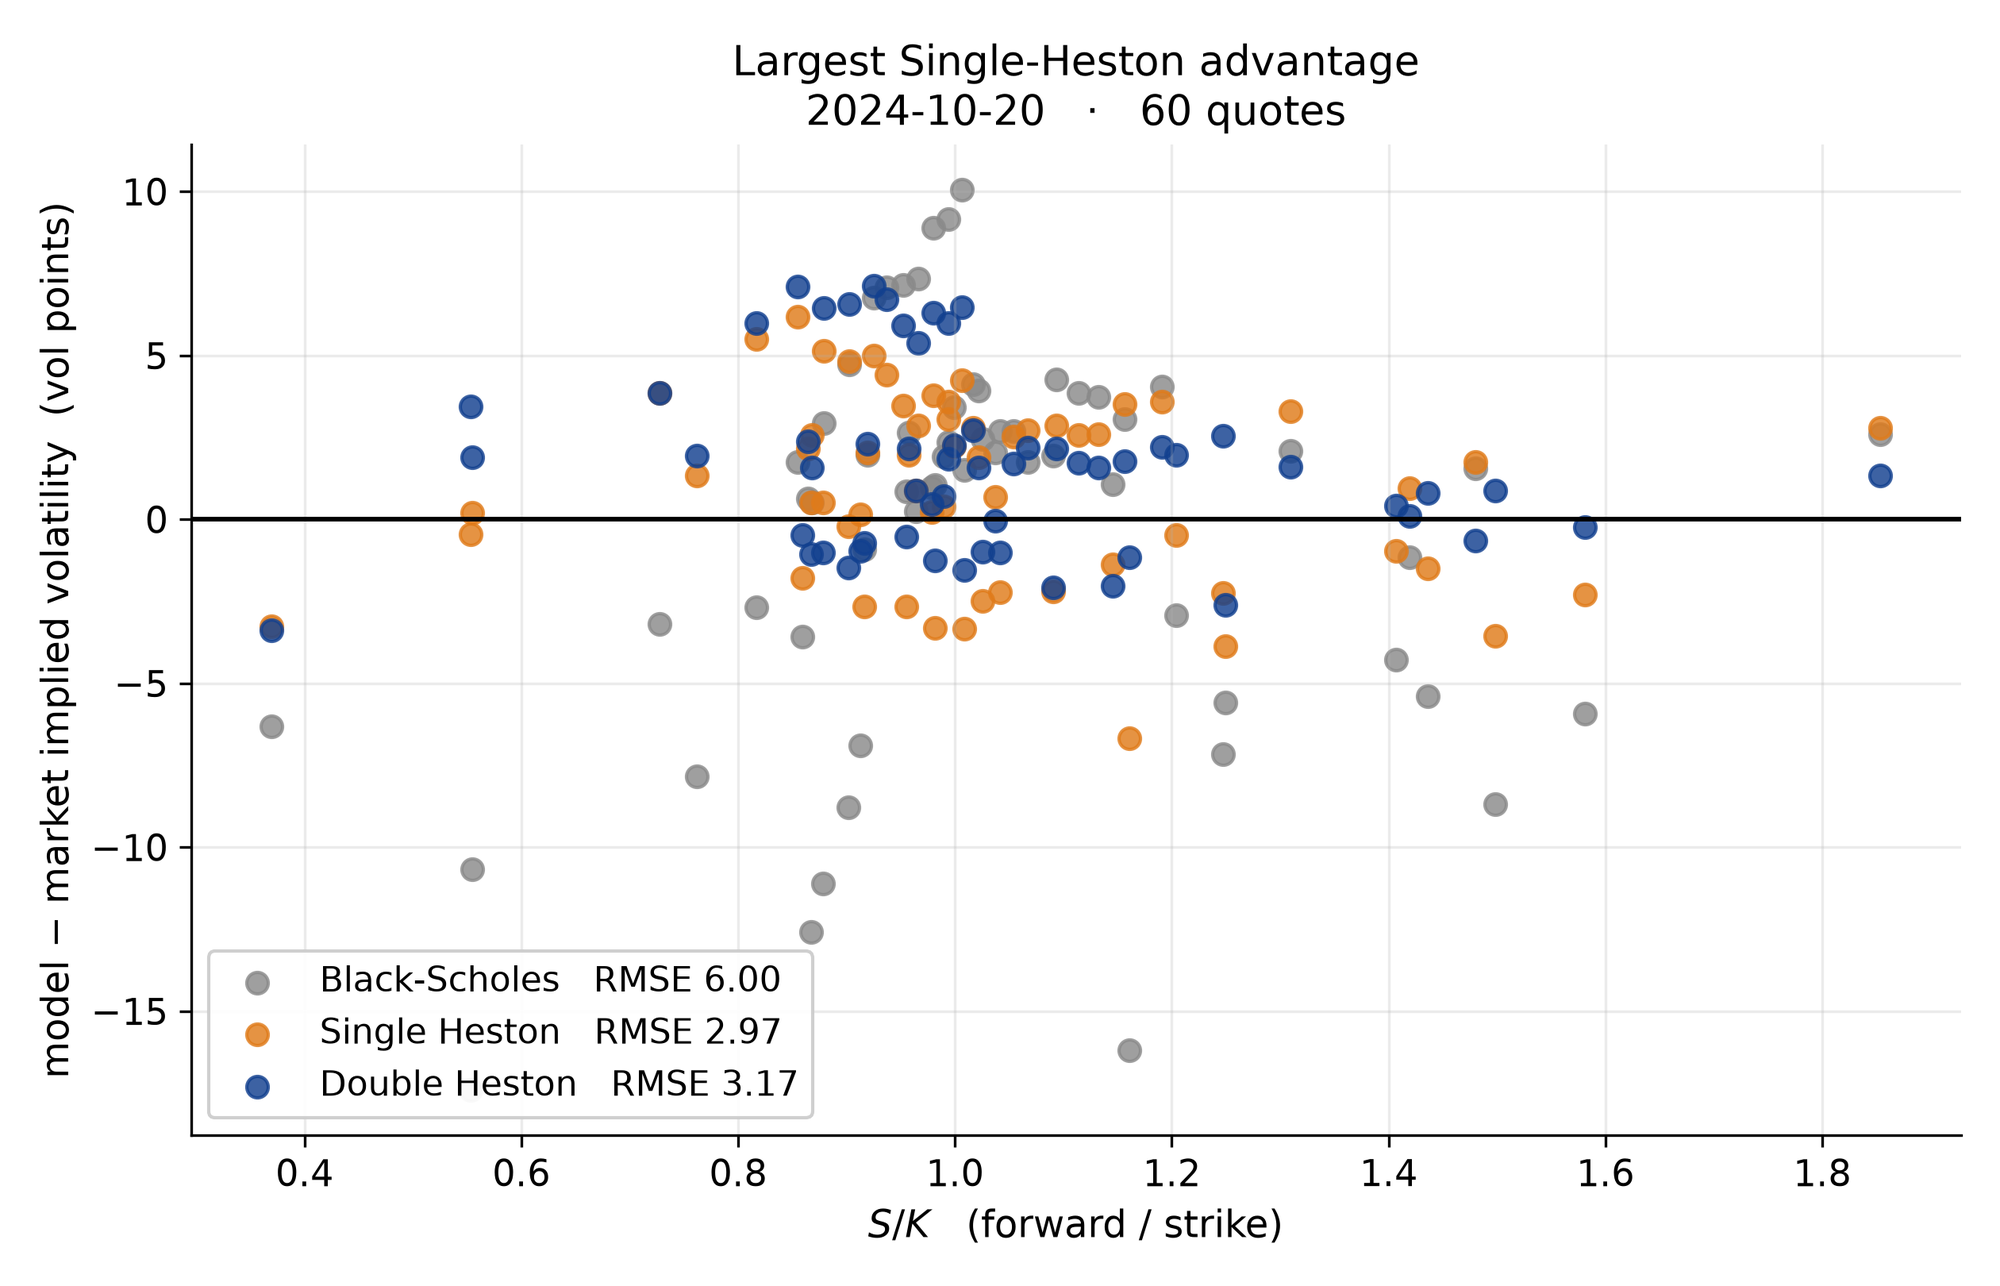
\includegraphics[width=0.85\linewidth]{fig_range_worst.png}
\caption{The supplied Bitcoin date on which Single Heston has the
greatest advantage (20 October 2024; 60 quotes), using an enlarged crop
from the original source. As in the preceding figure, the vertical
measure is model minus market implied volatility in volatility points.
Shown to avoid relying on favourable examples alone.}
\label{fig:worst}
\end{figure}

\FloatBarrier

% =====================================================================
\section{Discussion}
\label{sec:discussion}

Under the stated two-part, direction-specific criterion, the reported
comparison favours Double Heston over Single Heston in Bitcoin and Ether
but not in the remaining three markets. These results are cellwise and
the multiple-testing treatment is not documented. The correspondence
with quoted maturity coverage motivates further investigation of factor
identifiability, rather than demonstrating a universal expiry-count
threshold. Liquidity, strike coverage, calibration bounds and market
history may also affect the comparison. In particular, the Solana
calm-date mean difference and bootstrap interval favour Single Heston,
but a reverse-direction confirmatory Wilcoxon test was not supplied. The
results therefore motivate checking how much model complexity each
observed surface can support.

% =====================================================================
\section{Limitations}
\label{sec:limitations}

One feature of the sampling bears directly on the central variable. A date
enters the sample only if it quotes a minimum number of distinct expiries, and
that minimum was set to five for Bitcoin and Ether but to four for Solana, XRP
and Hyperliquid, because a common threshold of five would have excluded most
of the three thinner markets. The expiry-count contrast in
Table~\ref{tab:markets} is therefore measured under inclusion rules that are
not identical across markets, and part of the gap between six-to-seven and
about four expiries per day is induced by those rules rather than observed
freely. The direction of the effect is conservative with respect to the thin
markets, since a common threshold of five would have removed their least rich
surfaces and raised their median expiry count, but the grouping cannot be
claimed independent of the filter and a replication should fix one threshold
across all markets.

The study covers cryptocurrency options on a single venue (Deribit).
These markets differ in expiry coverage, liquidity and history. The
observed six-to-seven versus four-expiry grouping should not be
interpreted as a universal threshold, nor does pricing-error comparison
alone establish unique recovery of the two mean-reversion speeds.

Expiry count is not the only difference between these markets. Bitcoin
and Ether are also older, more liquid and have longer option histories.
With five markets we cannot fully separate maturity coverage from
liquidity, and we do not claim to. Expiry count is the variable that
identifiability theory singles out, and it orders the results without
exception, but a larger cross-section would be needed to isolate it.

The supplied manuscript reports neither the full quote-to-forward
conversion and filtering code nor calibration bounds, optimization logs,
date-by-expiry splits or clusterwise test vectors. The plotted Bitcoin
subset contains fewer dates and quotes than the table's BTC sample, and
its selection rule is not specified. The original maturity plot was
excluded because its visible jump is not accounted for by the stated
interpolation. The title refers to a physics-informed inverse-calibration
contribution, but the supplied experiments only evaluate direct
numerical fits: there is no trained inverse network, physics residual
objective, parameter-recovery ground truth, seed-wise stability or
uncertainty/identifiability experiment in the evidence package.

Hyperliquid has the shortest history of the five markets: its 55
evaluation dates fall inside one short listing window and are clustered
by ISO week rather than by volatility episode, so its 13 clusters are
less independent than the episode clusters used elsewhere. Our
calibration bounds bind in a large share of fits: the
volatility-of-variance upper bound is reached in 63 of 132 one-factor
fits (48\%), and in 80 of 132 (61\%, slow factor) and 76 of 132 (58\%,
fast factor) two-factor fits. Relaxing those bounds after seeing the
results is not permitted under our own protocol, so we record it as the
leading candidate improvement for a future, independently pre-registered
experiment. Finally, we measure pricing accuracy on held-out quotes from
the same day; forecasting, hedging performance and economic value are
separate questions.

% =====================================================================
\section{Conclusion}
\label{sec:conclusion}

The supplied evaluation reports a three-model direct-calibration
comparison across 16,186 option observations from five cryptocurrency
markets. The stated model medians show lower error for Double Heston
than the maturity-dependent Black baseline in all nine displayed rows.
The reported cluster-level directional criterion classifies Double
Heston as superior to Single Heston for Bitcoin and Ether, but not for
Solana, XRP and Hyperliquid. The association with quoted maturity
coverage is suggestive, not proof of a universal expiry threshold,
parameter identifiability, or causal model advantage. A research claim
about physics-informed inverse parameter recovery and its stability
requires separate neural-method and recovery experiments that are not
provided by this benchmark. The report should be supplemented with
prediction-level results, protocol provenance and validation of the
omitted maturity plot before stronger claims are made.

% =====================================================================
\begin{thebibliography}{99}

\bibitem{ref:bs}
Black, F., Scholes, M.: The pricing of options and corporate
liabilities. J. Polit. Econ. \textbf{81}(3), 637--654 (1973)

\bibitem{ref:merton}
Merton, R.C.: Theory of rational option pricing. Bell J. Econ. Manag.
Sci. \textbf{4}(1), 141--183 (1973)

\bibitem{ref:black76}
Black, F.: The pricing of commodity contracts. J. Financ. Econ.
\textbf{3}(1--2), 167--179 (1976)

\bibitem{ref:gatheral}
Gatheral, J.: The Volatility Surface: A Practitioner's Guide. Wiley,
Hoboken (2006)

\bibitem{ref:heston}
Heston, S.L.: A closed-form solution for options with stochastic
volatility with applications to bond and currency options. Rev. Financ.
Stud. \textbf{6}(2), 327--343 (1993)

\bibitem{ref:bakshi}
Bakshi, G., Cao, C., Chen, Z.: Empirical performance of alternative
option pricing models. J. Finance \textbf{52}(5), 2003--2049 (1997)

\bibitem{ref:bates}
Bates, D.S.: Post-'87 crash fears in the S\&P 500 futures option market.
J. Econom. \textbf{94}(1--2), 181--238 (2000)

\bibitem{ref:duffie}
Duffie, D., Pan, J., Singleton, K.: Transform analysis and asset pricing
for affine jump-diffusions. Econometrica \textbf{68}(6), 1343--1376
(2000)

\bibitem{ref:chj}
Christoffersen, P., Heston, S., Jacobs, K.: The shape and term structure
of the index option smirk: why multifactor stochastic volatility models
work so well. Manag. Sci. \textbf{55}(12), 1914--1932 (2009)

\bibitem{ref:carrmadan}
Carr, P., Madan, D.B.: Option valuation using the fast Fourier
transform. J. Comput. Finance \textbf{2}(4), 61--73 (1999)

\bibitem{ref:fangoost}
Fang, F., Oosterlee, C.W.: A novel pricing method for European options
based on Fourier-cosine series expansions. SIAM J. Sci. Comput.
\textbf{31}(2), 826--848 (2008)

\bibitem{ref:lordkahl}
Lord, R., Kahl, C.: Complex logarithms in Heston-like models. Math.
Finance \textbf{20}(4), 671--694 (2010)

\bibitem{ref:cui}
Cui, Y., del Ba\~{n}o Rollin, S., Germano, G.: Full and fast calibration
of the Heston stochastic volatility model. Eur. J. Oper. Res.
\textbf{263}(2), 625--638 (2017)

\bibitem{ref:feller}
Feller, W.: Two singular diffusion problems. Ann. Math. \textbf{54}(1),
173--182 (1951)

\bibitem{ref:madan}
Madan, D.B., Reyners, S., Schoutens, W.: Advanced model calibration on
bitcoin options. Digit. Finance \textbf{1}, 117--137 (2019)

\bibitem{ref:lian}
Lian, Y.-M., Chen, J.-H.: Pricing virtual currency-linked derivatives
with time-inhomogeneity. Int. Rev. Econ. Finance \textbf{71}, 424--439
(2021). \url{https://doi.org/10.1016/j.iref.2020.09.015}

\bibitem{ref:hou}
Hou, A.J., Wang, W., Chen, C.Y.H., H\"{a}rdle, W.K.: Pricing
cryptocurrency options. J. Financ. Econom. \textbf{18}(2), 250--279
(2020)

\bibitem{ref:ai2021}
Alexander, C., Imeraj, A.: The Bitcoin VIX and its variance risk
premium. J. Altern. Invest. \textbf{23}(4), 84--109 (2021)

\bibitem{ref:ai2023}
Alexander, C., Imeraj, A.: Delta hedging bitcoin options with a smile.
Quant. Finance \textbf{23}(5), 799--817 (2023)

\bibitem{ref:wilcoxon}
Wilcoxon, F.: Individual comparisons by ranking methods. Biom. Bull.
\textbf{1}(6), 80--83 (1945)

\bibitem{ref:efron}
Efron, B.: Bootstrap methods: another look at the jackknife. Ann. Stat.
\textbf{7}(1), 1--26 (1979)

\bibitem{ref:cameron}
Cameron, A.C., Gelbach, J.B., Miller, D.L.: Bootstrap-based improvements
for inference with clustered errors. Rev. Econ. Stat. \textbf{90}(3),
414--427 (2008)

\bibitem{ref:nosek}
Nosek, B.A., Ebersole, C.R., DeHaven, A.C., Mellor, D.T.: The
preregistration revolution. Proc. Natl. Acad. Sci. \textbf{115}(11),
2600--2606 (2018)

\bibitem{ref:raissi}
Raissi, M., Perdikaris, P., Karniadakis, G.E.: Physics-informed neural
networks: A deep learning framework for solving forward and inverse
problems involving nonlinear partial differential equations. J. Comput.
Phys. \textbf{378}, 686--707 (2019).
\url{https://doi.org/10.1016/j.jcp.2018.10.045}

\bibitem{ref:hainaut}
Hainaut, D., Casas, A.: Option pricing in the Heston model with physics
inspired neural networks. Ann. Finance \textbf{20}(3), 353--376 (2024).
\url{https://doi.org/10.1007/s10436-024-00452-7}

\bibitem{ref:zhang}
Zhang, C., Amici, G., Morandotti, M.: Calibrating the Heston model with
deep differential networks. Decisions Econ. Finance (2025).
\url{https://doi.org/10.1007/s10203-025-00558-1}

\end{thebibliography}

\end{document}
